%Example of use of oxmathproblems latex class for problem sheets
\documentclass{oxmathproblems}

%(un)comment this line to enable/disable output of any solutions in the file
%\printanswers

%define the page header/title info
\oxfordterm{CPS 824}
\course{Reinforcement Learning}
\sheetnumber{Assignment 1}
\sheettitle{Noah Mifsud-Lattari - 500760404}
% add further contact details to footer if desired,
%e.g. email address, or name and email address



\begin{document}

\begin{questions}

\miquestion
\begin{parts}

% 1 a)
  \part If the policy was set to $r_s = 1$ the agent may just repeatedly go between squares over and over to generate a high reward, gaining 1 point for every square traveled. This would have the program run infinitely and risk the green square never being located. 
  
  If the reward for the basic squares was set to a punishment like $r_s = -1$, the program can find the shortest path eventually. In this approach, the program is getting a penalty for taking longer to get to the green square. After training the optimal policy should figure out a quick path to the green square from any square without any redundant squares.
  
  let $r_g = 5$,  $r_r = -5$,  $\gamma = 1$  and $r_s = -1$. The optimal policy values for the puzzle would look like the following: 
\\
  \[\pi_g = \begin{pmatrix}
    0 & 1 & 2 & 3\\
    -5 & 2 & 3 & 4 \\
    2 & 3 & 4 & 5 \\
    1 & 0 & -1 & -2 \\
\end{pmatrix} \]


% 1 b)
  \part If each reward has +2 added to them, the rewards are now: $r_g = 7$, $r_r = -3$, and $r_s = 1$. The optimal policy will now have this set of values:
\\
  \[\pi_g =\begin{pmatrix} 
    12 & 11 & 10 & 9\\
    -3 & 10 & 9 & 8 \\
    10 & 9 & 8 & 7 \\
    11 & 12 & 13 & 14 \\
\end{pmatrix} \]


% 1 c)
  \part n/a


% 1 d)
  \part As mentioned in 1 (a), a positive reward (such as $r_s = 2$) would potentially cause problems in finding the optimal path. Since the program’s goal is to maximize the current reward, it may constantly go back and forth from squares in order to generate a high reward. This would potentially lead to failure as there is a chance the program never finds the green square.

  
% 1 e)
 \part Yes, it can change and does depend on the choice of gamma. A small discount factor would eventually find the optimal path to the green square because the rewards in the future would be worth less than present rewards.


% 1 f)
 \part If you chose a comically small reward value like $r_s = -500$, we could end up at the red square because each normal square would yield a reward of -500, while the red square would yield a reward of -5. Since the program’s job is to maximize the reward, it will eventually form a path to the red square.
\\ 
\end{parts}


\miquestion
\begin{parts}
% 2 a)
  \part See code.

% 2 b)
  \part See code.

% 2 c)
 \part The results from running both the deterministic \& the stochastic environment for 200 iterations are pictured below. For the first environment, the program always succeeded in finding the policy with a rate of 1.0 (100\%) and ran quite quickly. The stochastic method had a success rate of around 70\%, (140 successes / 200 iterations). This is due to the randomness factor of the stochastic environment, and the potential for the program to slip on the ice by chance. It took me about 1 hour to finish.
\\ \\
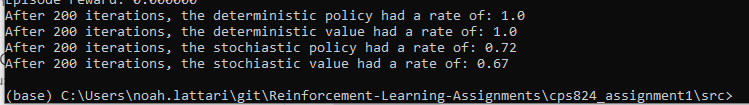
\includegraphics[scale=0.757]{iters.png} 
\end{parts}


\end{questions}

\end{document}
